\documentclass{article}
\usepackage[slovak]{babel}
\usepackage[utf8]{inputenc}

\usepackage{indentfirst}
\usepackage{graphicx}

\begin{document}
    \begin{titlepage}
        \begin{center}
            \vspace{\stretch{0.382}}
            
            
\includegraphics[width=10cm]{FITlogo.png}\\[30mm]
            
            \LARGE
            Implementácia prekladača imperatívneho jazyka IFJ17 \\
            \large
            Dokumentácia k~projektu IFJ/IAL\\[55mm]
            
            \begin{tabular}{r l l}
                Tím: & 094 & \\
                Varianta: & II & \\
                Vedúci: & Tomáš Nereča (xnerec00) & 26\% \\
                Ďalší členovia: & Samuel Obuch (xobuch00) & 26\% \\
                    & Jiří Vozár (xvozar04) & 26\% \\
                    & Ján Farský (xfarsk00) & 22\% \\
                Implementované rozšírenia: & BASE, FUNEXP, IFTHEN &\\
            \end{tabular}
            
            \vspace{\stretch{0.618}}
        \end{center}
    \end{titlepage}

    \tableofcontents
        \thispagestyle{empty}
        \newpage
        \setcounter{page}{1}
    \newpage
    
    \section{Úvod}
        Dokumentácia popisujúca implementáciu prekladača imperatívneho jazyka IFJ17. Prekladač načítava
        zdrojový kód jazyka IFJ17 zo~štandardného vstupu a ten pomocou lexikálnej, syntaktickej a sémantickej
        analýzy vyhodnotí a vygeneruje potrebné inštrukcie v~IFJcode17 pre interpret. V~prípade
        výskytu chyby pri analýze kódu IFJ17 prekladač vráti kód príslušnej chyby a chybové hlásenie na štandardný
        chybový výstup.
        
        Dokumentácia taktiež zahŕňa zhodnotenie práce v~tíme a približuje logiku a fungovanie
        jednotlivých častí prekladača. 
    
    \section{Implementácia}
    
        \subsection{Lexikálna analýza}
        Hlavná funkcia lexikálneho analyzátora je \texttt{getNextToken}. Je implementovaná v súbore \emph{scanner.c}.
        Jej argumenty sú ukazatele na štruktúru typu \texttt{tToken} a \texttt{FILE} a jej návratový typ je \texttt{bool}. 

        Funkcia číta lexémy zo zadaného súboru(spravidla \texttt{stdin}). Lexémy sú spracované pomocou konečného automatu. 
        Ak sa automat dostane do konečného stavu, funkcia vráti hodnotu \texttt{true} a podľa spracovaných lexém nastaví
        token predaný v argumente. Ak nastane počas lexikálnej analýzy chyba, vráti funkcia hodnotu \texttt{false} a 
        token nenastavuje. 

        Dátová štruktúra \texttt{tToken} a jej podštruktúry sú definované v hlavičkovom súbore \emph{scanner.h}. 
        Platný token musí mať vždy definovaný typ. V prípade, že to typ tokenu vyžaduje tak aj atribút 
        (napr. načítaný reťazec v prípade, že je token typu \texttt{string}). 

        Funkcia \texttt{getNextToken} sa taktiež stará o prevod veľkých písmen na malé a počítanie riadkov.
        Taktiež uľahčuje prácu syntaktickému analyzátoru, pretože rozlišuje medzi identifikátormi a kľučovými slovami.
        V poli reťazcov sú uložené všetky kľúčové slová a \emph{binárnym vyhľadávaním} vo funkcii \texttt{identifierTest} 
        sa testuje, či sa jedná o identifikátor alebo kľúčové slovo.

        Diagram konečného automatu nájdete v prílohe.

        \subsection{Syntaktická analýza}
            Prekladač využíva syntaxou riadený preklad, v ktorom kombinuje \emph{rekurzívny zostup} pre základné konštrukcie
            a príkazy jazyka s \emph{precedenčnou syntaktickou analýzou} pre výrazy.
            Vstupným bodom prekladača je funkcia \texttt{parse}, ktorá zavolá vyhodnotenie hlavného neterminálu \emph{program},
            ktorý po kontrole volá funkcie z neho vychádzajúcich ďalších neterminálov.
            Pokiaľ pravidlo očakáva výraz, je zavolaná funkcia \texttt{expression}, ktorá se postará o vyhodnotenie výrazu prevodom
            do postfixovej podoby.
            
            \subsubsection{Rekurzívny zostup}
                Pre každý neterminál je vytvorená funkcia, ktorá je volaná pre vyhodnotenie daného neterminálu.
                Funkcia potom vracia hodnotu \texttt{true}, pokiaľ bolo vyhodnotenie úspešné a hodnotu \texttt{false}, pokiaľ došlo k nejakej chybe. Niektoré funkcie z dôvodu zjednodušenia nereprezentujú pravidlá úplne presne, kedy se napríklad funkcia \texttt{statementList} nevolá rekurzívne, ale je riadená cyklom. Samotný zostup je rozdelený do 3 modulov pre oddelenie všeobecných neterminálov, neterminálov príkazov a neterminálov funkcií.
            
            \subsubsection{Precedenčná syntaktická analýza}
                Precedenčná syntaktická analýza je založená na precedenčnej tabuľke a prevode infixových výrazov
                na postfix, z ktorého sú následne generované inštrukcie IFJcode17. 

                Pri nájdení výrazu je zavolaná funkcia \texttt{expression}, ktorá ako argument dostane očakávaný
                výstupný typ tokenu. Na základe tohoto očakávaného tokenu kontrolujeme pri vytváraní \emph{postfixového 
                výrazu} pomocou funkcie \texttt{postfix} povolené dátové typy vo výraze. 

                Na každý token je zavolaná funkcia \texttt{getTerm}, ktorá v prípade ak sa vo výraze nachádza premenná 
                alebo volanie funkcie overí, či boli deklarované. Ďalej funkcia vracia index tokenu z precedenčnej tabuľky 
                a typ spracovaného tokenu v štruktúre typu tTerm. Ak vyhodnotenie operandu alebo operácie vo funkcii 
                \texttt{postfix} prebehlo korektne, je zavolaná funkcia \texttt{generateInstruction} na vygenerovanie 
                inštrukcie pre daný tTerm. 

                Funkcia \texttt{postfix} spracúva dalšie tokeny až pokým nenarazí na koniec výrazu. 
                Pri vytváraní postfixového výrazu využíva abstraktný dátový typ \texttt{tStack} na dočasné ukladanie 
                premenných typu \texttt{tTerm}. 

                Ak preklad na \emph{postfix} prebehol úspešne funkcia \texttt{expression} vracia hodnotu \texttt{true}, 
                v prípade chyby sa vypíše chybové hlásenie a funkcia vracia hodnotu \texttt{false}.
    
        \subsection{Tabuľka symbolov}
            Tabuľka symbolov je implementovaná ako hash tabuľka. Hashovacia funkcia bola zvolená \emph{djb2}\footnote{\texttt{http://www.cse.yorku.ca/\~{}oz/hash.html}}, pretože dávala dobré výsledky rozloženia pri experimentovaní s väčším množstvom záznamov.
            
            Veľkosť poľa pre ukazatele bola zvolená $128$ aby sa operácia modulo v hashovacej funkcii previedla na bitové maskovanie a pre bežný počet premenných vo funkcii je veľkosť poľa dostačujúca.
            
            Informácie o symbole sú následne ukladané v štruktúre, ktorá bola navrhnutá univerzálne pre informácie o premenných aj funkciách.
        
        \subsection{Vstavané funkcie}
            V prekladači sme implementovali aj štyri vstavané funkcie jazyka IFJ17 a to \textbf{Length, Chr, Asc} a \textbf{Substr}.
            Funkcie sme implementovali v module ifunc. Ak funkcia \texttt{expression} pri vyhodnocovaní výrazu narazí na volanie 
            niektorej zo vstavaných funkcií, zavolá si konkrétnu funkciu z modulu ifunc. Tá si následne spracuje argumenty a 
            vygeneruje potrebné inštrukcie. Vstavané funkcie pracujú s premennými na globálnom rámci, ktoré sú vytvorené pri štarte programu.

            \paragraph{Length}
            Pomocou inštrukcie \emph{STRLEN} sa získa dĺžka reťazca. Je potrebné použiť pomocné premenné, pretože 
            inštrukcia \emph{STRLEN} nemá zásobníkovú variantu.

            \paragraph{Chr}
            Pomocou zásobníkovej inštrukcie \emph{INT2CHARS} sa jednoducho prevedie zadané číslo z ascii tabuľky na znak.

            \paragraph{Asc}
            Po kontrole argumentov pomocou inštrukcií \emph{GT} a \emph{LT} sa buď skočí na návestie pomocou inštrukcie 
            \emph{JUMP} (v tomto prípade vráti funkcia hodnotu 0), alebo sa vykoná inštrukcia \emph{STRI2INT},
            ktorá prevedie zadaný znak na požadovanom indexe na číslo z ascii tabuľky.

            \paragraph{SubStr}
            Riešenie tejto funkcie bolo zložitejšie, pretože inštrukčná sada neobsahuje inštrukciu pre získanie podreťazca. 
            Po kontrole argumentov podobne ako pre funkciu \textbf{Asc}, sa v cykle tvoril výstupný reťazec
            pomocou konkatenácie vždy jedného znaku na koniec výstupného reťazca. K tomu sme využili inštrukcie ako napríklad
            \emph{ADD} pre inkrementovanie počítadla, \emph{JUMPIFEQ} pre skok na začiatok cyklu, \emph{GETCHAR} 
            pre získanie znaku z reťazca alebo \emph{CONCAT} pre pripojenie znaku na koniec reťazca.
            
        \subsection{Generovanie kódu}
            Cieľový kód je generovaný priamo počas jediného priechodu vypisovaním príslušných inštrukcií vo funkcii
            príslušného pravidla.
            
            Premenné definované užívateľom sa ukladajú na dátový rámec, ktorý sa pre funkcie tvorí vždy nový.
            Výrazy využívajú pre medzivýsledky zásobník, kam sa ukladajú aj vyhodnotené parametre a výsledky funkcií.
            
            Podmienky a cykly využívajú inštrukcie podmienených a nepodmienených skokov, ale funkcie se volajú inštrukciami \texttt{CALL}
            a \texttt{RETURN}.
        
    \section{Rozšírenia}
    Boli implementované celkom 3 rozšírenia
        \begin{itemize}
            \item \textbf{base}   - Lexikálny analyzátor dokáže prečítať celé číslo zadané v inej než
                                    desiatkovej sústave a následne ho previesť pomocou funkcie 
                                    \emph{strtol} s argumentom príslušnej číselnej sústavy do \emph{integeru}.
            \item \textbf{funexp} - Vďaka vhodnému návrhu nezávislého vyhodnocovania výrazov a predávaní parametrov funkcií
                                    cez zásobník ako výsledky rekurzívne volaných podvýrazov bolo toto rozšírenie implementované
                                    už v základnej verzii prekladača.
            \item \textbf{ifthen} - Podpora \emph{elseif} a možnosť vynechania \emph{else} obnášala iba jednoduchú úpravu funkcie
                                    pre vyhodnocovanie podmienok prepísaním do cyklu a rozšírením generovania inštrukcií
                                    pre skoky a návestia.
        \end{itemize}
    
    \section{Testovanie}
    Na začiatku sme určili jedného člena, ktorý písal jednotkové testy pre lexikálny analyzátor.
    Jednotkové testy boli napísané v jazyku C. Na testovací súbor, ktorý obsahoval rôzne tokeny bola volaná funkcia
    \texttt{getNextToken}. Následne prebiehala kontrola, či lexikálny analyzátor určil správny typ a prípadne atribút
    jednotlivých tokenov.
    
    Neskôr sme napísali zopár vlastných regresných testov, tieto testy sme už písali v jazyku \emph{Python}, kde
    sme na vstup nášho prekladača posielali zdrojový kód IFJ17, jeho výstup v prípade ak nenastala chyba sme posielali
    do interpretu a výstup interpretu sme uložili do súboru. Na záver sme porovnali očakávaný výstup so získaným výstupom
    z interpretu alebo chybovým hlásením z prekladača. Ak sa výstupy zhodovali test prebehol úspešne ak nie test zlyhal.
    
    Využívali sme aj verejnú databázu testov našich kolegov, do ktorej sme neskôr prispievali vlastnými testami. 
    To nám pomohlo čo najrobustnejšie otestovať funkčnosť nášho prekladača.
    
    \section{Práca v~tíme}
    Ako tím sme sa začali schádzať prakticky ihneď po zaregistrovaní nášho zadania. Stretávali sme sa 
    zvyčajne raz do týždňa. Vždy sme prediskutovali aktuálny stav práve implementovaných častí 
    a ďalší postup či korekcie v~zdrojovom kóde. Ako komunikačný kanál sme využívali prevažne 
    skupinovú konverzáciu na sociálnej sieti Facebook. Bolo to jednoduché a efektívne riešenie.

    Prácu sme sa snažili rozdeľovať rovnomerne medzi všetkých členov tímu, čo sa nám nepodarilo vždy. 
    Po pridelení úlohy sme stanovili deadline, aby sme mohli čo najskôr pokračovať na nasledujúcej časti projektu. 
    Jednotlivé časti sme sa snažili implementovať paralelne s~preberanou látkou na prednáškach, aby sme sa vyhli chybám z dôvodu neznalosti.
    

        \subsection{Správa zdrojového kódu}
        Pre správu a zdielanie zdrojových súborov sme využili verzovací systém \emph{Git} a webovú službu GitHub pre vzdialené ukladanie, ktorú sme už počas štúdia využili na verzovanie projektov v~iných predmetoch.
        
        Na sledovanie postupu pri plnení pridelených úloh a oznamovanie nájdených chýb 
        sme využívali nástroj Trello, ktorý slúži ako online kanban pre sledovanie projektov. 
        
        Vďaka týmto informačným kanálom mohli mať všetci členovia tímu prístup k~najaktuálnejšej
        verzii projektu a reagovať na vzniknuté chyby efektívne.

        \subsection{Rozdelenie práce v tíme}

        \textbf{Tomáš Nereča} pracoval na implementácii lexikálneho analyzátora a v neskoršej fáze vývoja pomáhal pri implementácii niektorých
        funkcií precedenčnej syntaktickej analýzy. Okrem toho sa podieľal na menších moduloch symtable, errors, stack a ifunc.  

        \textbf{Jiří Vozár} mal na starosti vedenie implementácie, návrh komunikácie medzi modulmi a implementáciu syntaktickej analýzy rekurzívnym zostupom.

        \textbf{Samuel Obuch} pracoval na implementácii precedenčnej syntaktickej analýzy, vytvoril regresné testy a vypracoval pomocný modul strings pre lexikálny analyzátor.

        \textbf{Ján Farský} vypracoval základné jednotkové testy pre lexikálny analyzátor, vytvoril precedenčnú tabuľku, pracoval na module ifunc a napísal základ dokumentácie.

        Dôvodom nerovnomerného rozdelenia bodov bolo nedostatočné splnenie úloh jedného 
        z~členov tímu, čo viedlo k nutnosti zapojiť k týmto úlohám iných členov tímu.

    \section{Záver}
    S~projektom podobného rozsahu sa ešte nikto z~nás predtým nestretol, preto ho považujeme za dobrú
    skúsenosť pre každého z~nás. Pri jeho riešení sme prakticky využili získané vedomosti z~predmetov 
    IFJ a IAL.
    
    Pre správne fungovanie tímu bolo potrebné kvalitné riadenie a pridelovanie úloh a pravideľná
    komunikácia medzi jednotlivými členmi tímu. Výsledkom tejto práce je funkčný a z~nášho pohľadu vydarený 
    prekladač jazyka IFJ17.
    
    \newpage
    \section{Prílohy}
        \subsection{Diagram konečného automatu}
            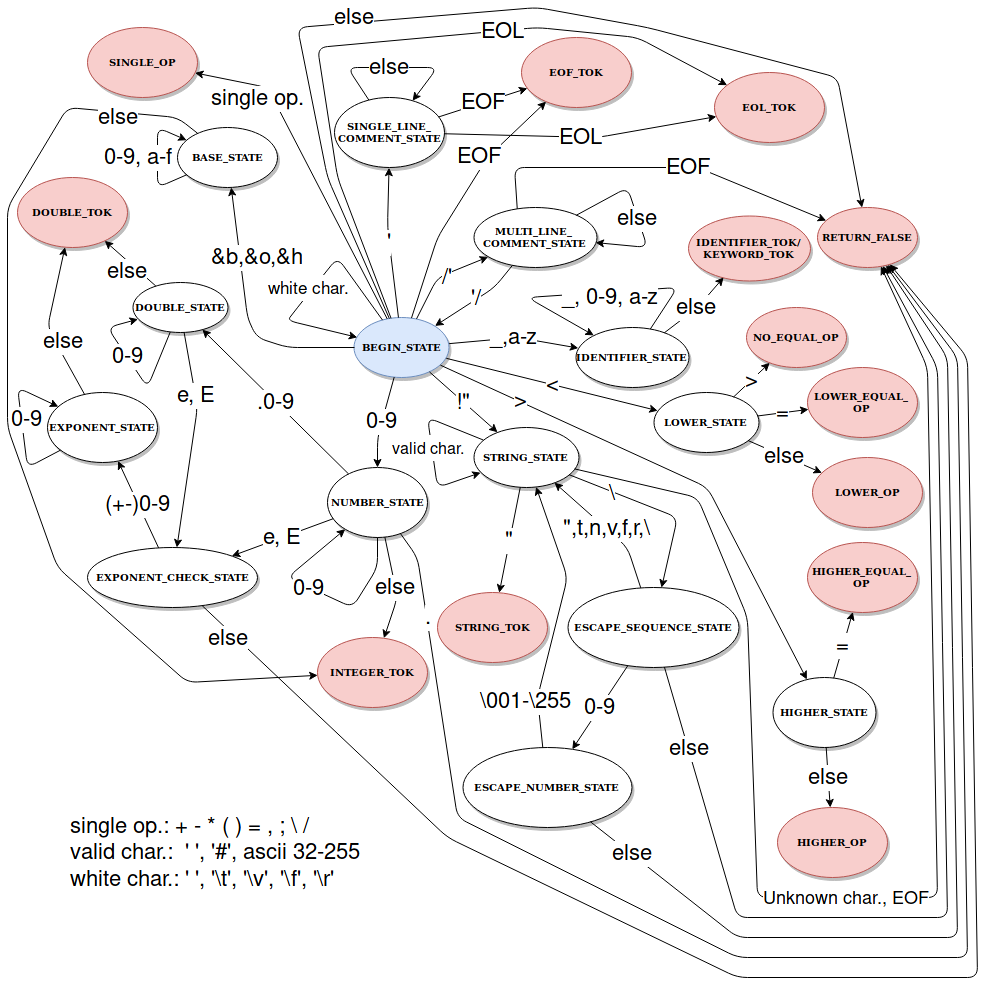
\includegraphics[trim=6cm 0 0 0, width=15cm]{finite_automata.png}
            \newpage
            
        \subsection{LL gramatika}
            \begin{enumerate}
                % NESAHAT - zhenodnotí čísla v tabulce LL gramatiky!
                \item \texttt{<program> -> declare function <functionDecl> eol <program>}
                \item \texttt{<program> -> function <functionDef> eol <program>}
                \item \texttt{<program> -> scope <statementList> end scope}
                
                \item \texttt{<functionDecl> -> <functionHeader>}
                \item \texttt{<functionDef> -> <functionHeader> eol <statementList> end function}
                
                \item \texttt{<functionHeader> -> identifier ( <functionParams> ) as type}
                
                \item \texttt{<functionParams> -> <functionParam> <nextFuncParam>}
                \item \texttt{<functionParams> -> epsilon}
                
                \item \texttt{<nextFuncParam> -> , <functionParam> <nextFuncParam>}
                \item \texttt{<nextFuncParam> -> epsilon}
                
                \item \texttt{<functionParam> -> identifier as type}
                
                \item \texttt{<statementList> -> <statement> eol <statementList>}
                \item \texttt{<statementList> -> epsilon}
                
                \item \texttt{<statement> -> dim <declaration>}
                \item \texttt{<statement> -> identifier = <expression>}
                \item \texttt{<statement> -> input identifier}
                \item \texttt{<statement> -> print <printArgs>}
                \item \texttt{<statement> -> if <expression> then eol <statementList> <else>}
                \item \texttt{<statement> -> do while <expression> eol <statementList> loop}
                \item \texttt{<statement> -> return identifier}
                
                \item \texttt{<declaration> -> identifier as type}
                \item \texttt{<declaration> -> identifier as type = <expression>}
                
                \item \texttt{<printArgs> -> <expression> ;}
                \item \texttt{<printArgs> -> <expression> ; <printArgs>}
                
                \item \texttt{<else> -> elseif <expression> then eol <else> end if}
                \item \texttt{<else> -> else eol <statementList> end if}
                \item \texttt{<else> -> end if}
                
                \item \texttt{<expression> ->} vyhodnocuje se precedenční syntaktickou analýzou
            \end{enumerate}
        \newpage
        
        \subsection{LL tabuľka}
        \newcommand{\tterm}[1]{\rotatebox[origin=c]{90}{\texttt{#1}}}
            \begin{tabular}{|r|*{10}{c|}}
                \hline
                & \tterm{declare} & \tterm{function} & \tterm{scope} & \tterm{identifier} & \tterm{dim} &
                \tterm{input} & \tterm{print} & \tterm{if} & \tterm{do} & \tterm{return} \\\hline \hline
                \texttt{<program>} & 1 & 2 & 3 &&&&&&& \\\hline
                \texttt{<functionDecl>} &&&& 4 &&&&&& \\\hline
                \texttt{<functionDef>} &&&& 5 &&&&&& \\\hline
                \texttt{<functionHeader>} &&&& 6 &&&&&& \\\hline
                \texttt{<functionParams>} &&&& 7, 8 &&&&&& \\\hline
                \texttt{<nextFuncParam>} &&&&&&&&&& \\\hline
                \texttt{<functionParam>} &&&& 11 &&&&&& \\\hline
                \texttt{<statementList>} &&&& 12 & 12 & 12 & 12 & 12 & 12 & 12 \\\hline
                \texttt{<statement>} &&&& 15 & 14 & 16 & 17 & 18 & 19 & 20 \\\hline
                \texttt{<declaration>} &&&& 21, 22&&&&&& \\\hline
                \texttt{<else>} &&&& 23, 24&&&&&& \\\hline
            \end{tabular}
            
            \begin{tabular}{|r|*{9}{c|}}
                \hline
                & \tterm{elseif} & \tterm{else} & \tterm{end} & \tterm{loop} & \tterm{eol} &
                \tterm{(} & \tterm{)} & \tterm{=} & \tterm{,} \\\hline \hline
                \texttt{<program>} &&&&&&&&& \\\hline
                \texttt{<functionDecl>} &&&&&&&&& \\\hline
                \texttt{<functionDef>} &&&&&&&&& \\\hline
                \texttt{<functionHeader>} &&&&&&&&& \\\hline
                \texttt{<functionParams>} &&&&&&& 8 && \\\hline
                \texttt{<nextFuncParam>} &&&&&&& 10 && 9 \\\hline
                \texttt{<statementList>} & 13 & 13 & 13 & 13 &&&&& \\\hline
                \texttt{<statement>} &&&&&&&&& \\\hline
                \texttt{<declaration>} &&&&&& 23, 24&&& \\\hline
                \texttt{<else>} & 25 & 26 & 27 &&&&&& \\\hline
            \end{tabular}
        \newpage

        \subsection{Precedenčná tabuľka}

        \begin{center}
        \begin{tabular}{|c||c|c|c|c|c|c|c|c|c|c|c|c|c|c|c|c|c|c|}
        \hline
                    &  =  & $<>$ & $<$= & $>$= & $<$ & $>$ &  +  &  -  &  *   &  /  & \textbackslash &  (  &  )  & \$  \\ 
        \hline
        \hline  
           =        & $>$ &  $>$ &  $>$ &  $>$ & $>$ & $>$ & $<$ & $<$ &  $<$ & $<$ & $<$            & $<$ & $>$ & $>$ \\ 
        \hline  
          $<>$      & $>$ &  $>$ &  $>$ &  $>$ & $>$ & $>$ & $<$ & $<$ &  $<$ & $<$ & $<$            & $<$ & $>$ & $>$ \\
        \hline  
          $<$=      & $>$ &  $>$ &  $>$ &  $>$ & $>$ & $>$ & $<$ & $<$ &  $<$ & $<$ & $<$            & $<$ & $>$ & $>$ \\
        \hline  
          $>$=      & $>$ &  $>$ &  $>$ &  $>$ & $>$ & $>$ & $<$ & $<$ &  $<$ & $<$ & $<$            & $<$ & $>$ & $>$ \\
        \hline  
          $<$       & $>$ &  $>$ &  $>$ &  $>$ & $>$ & $>$ & $<$ & $<$ &  $<$ & $<$ & $<$            & $<$ & $>$ & $>$ \\
        \hline        
          $>$       & $>$ &  $>$ &  $>$ &  $>$ & $>$ & $>$ & $<$ & $<$ &  $<$ & $<$ & $<$            & $<$ & $>$ & $>$ \\
        \hline  
           +        & $>$ &  $>$ &  $>$ &  $>$ & $>$ & $>$ & $>$ & $>$ &  $<$ & $<$ & $<$            & $<$ & $>$ & $>$ \\
        \hline  
           -        & $>$ &  $>$ &  $>$ &  $>$ & $>$ & $>$ & $>$ & $>$ &  $<$ & $<$ & $<$            & $<$ & $>$ & $>$ \\ 
        \hline  
          */        & $>$ &  $>$ &  $>$ &  $>$ & $>$ & $>$ & $>$ & $>$ &  $>$ & $>$ & $>$            & $<$ & $>$ & $>$ \\ 
        \hline  
\textbackslash      & $>$ &  $>$ &  $>$ &  $>$ & $>$ & $>$ & $>$ & $>$ &  $<$ & $<$ & $>$            & $<$ & $>$ & $>$ \\
        \hline  
           (        & $<$ &  $<$ &  $<$ &  $<$ & $<$ & $<$ & $<$ & $<$ &  $<$ & $<$ & $<$            & $<$ &  =  &     \\  
        \hline  
           (        & $>$ &  $>$ &  $>$ &  $>$ & $>$ & $>$ & $>$ & $>$ &  $>$ & $>$ & $>$            &     & $>$ & $>$ \\ 
        \hline  
          \$        & $<$ &  $<$ &  $<$ &  $<$ & $<$ & $<$ & $<$ & $<$ &  $<$ & $<$ &  $<$            & $<$ &     &     \\ 
        \hline  
        \end{tabular}
    \end{center}
\end{document}